\documentclass[12pt]{article}
\usepackage{indentfirst}
\usepackage{amssymb}
\usepackage{amsmath}
\usepackage{color, xcolor}
\usepackage[ruled,vlined]{algorithm2e}
\usepackage{graphicx}

\usepackage{tikz-qtree}
\usetikzlibrary{calc}
\usetikzlibrary{shapes,arrows,chains}
\usetikzlibrary{automata,positioning}
\tikzset{edge from parent/.append style={<-}}
\tikzstyle{sn}=[circle, draw, align=center, fill=white!50, inner sep=0pt, minimum size=0.6cm]

\tikzstyle{kn}=[circle, draw, align=center, fill=white!50, inner sep=0pt,
minimum size=1.6cm]

\tikzstyle{fsn}=[circle, draw, fill=blue!30, inner sep=0pt, minimum size=0.6cm]

\begin{document}
	\pagestyle{empty}

	\begin{center}
		\vspace*{1.5cm}
		%\includegraphics[scale=0.5]{../common/Nebulas.png}
		\vspace{0.5cm}
		\textbf{\huge{Liquid Democracy}}

		\vspace{0.5cm}
		ASResearch
		\textbf{}
	\end{center}
\section{Problem Description}
Suppose there are $n$ voters, each voter has a certain amount of voting power $a[i],i=1,2,...,n$.

The liquid democracy refers that, each voter (called delegator) can delegate all his voting power to another voter (called delegatee), and his degegatee can further delegate all those voting power to another delegatee. Whenever a delegatee votes to a candidate, by default, all his delegators' (including multi-level) voting powers are also cast to that candidate.

We use a (direct) graph $G=(V,E)$ to represent the delegate relationship among
voters, where each note represents a voter, and a direct edge $(u,v)$
represents that voter $v$ delegates to voter $u$. Since by default there is no
loop in $G$, thus $G$ is a forest (multiple trees). For convenience, in the
case where there are more than one connect branch, we add a virtual node that
is pointed by the root of each branch. So $G$ is transferred to tree $T$, as
Figure~\ref{fig:1}.

That is, there are 12 voters, each node's  (voter) parent represents its
delegatee. As an example, now we  suppose $a[i]=i$. At the beginning, nobody
votes. When voter 1 votes for candidate $A$ (as the first voter), $A$ obtains
$1+2+...+12=78$ votes.

Meanwhile liquid democracy allows voters to change their votes when they are unsatisfied with the voting results of delegatees (including multilevel). Correspondingly, their delegatees' voting powers decrease.

As Figure~\ref{fig:1}, after voter 1 votes, suppose voter 5 (as the second
voter) votes for candidate $B$. Then $B$ obtains $6+5=11$ votes. $A$'s vote
decreases by 11, turning into 67.

Suppose further, voter 3 (the third voter) votes for candidate $C$, then $C$
obtains $3+4+7+8=22$ votes, $A$'s  vote become 45, and $B$'s vote is still 11.

\begin{figure*}
  \centering
	\label{fig:1}
	%\includegraphics[width=0.6\textwidth]{1.png}
	%\includegraphics[width=0.6\textwidth]{2.png}
	%
  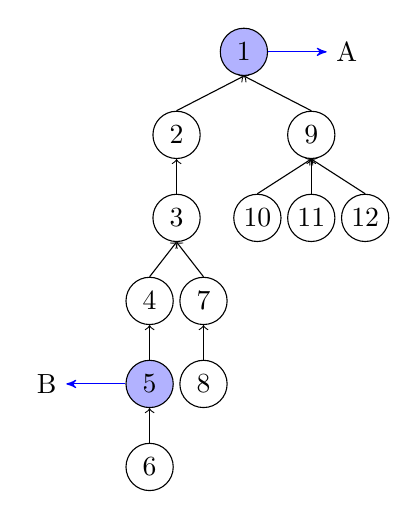
\begin{tikzpicture}
%\tikzset{grow'=right,level distance=32pt}
%\tikzset{execute at begin node=\strut}
%\tikzset{every tree node/.style={anchor=base west}}
\Tree
[.\node[fsn](n1){1};
  [.\node[sn]{2};
   [.\node[sn]{3};
    [.\node[sn]{4};
     [.\node[fsn](n5){5};
      [.\node[sn]{6};]]]
    [.\node[sn]{7};
     [.\node[sn](n8){8};]]] ]
  [.\node[sn]{9};
   [.\node[sn]{10};]
   [.\node[sn]{11};]
   [.\node[sn]{12};]]
]
\node (a) at ($(n1.east) + (1, 0)$) {A};
\node (b) at ($(n5.west) + (-1, 0)$) {B};
\draw [->, >=stealth', color=blue] (n1) -- (a);
\draw [->, >=stealth', color=blue] (n5) -- (b);

\end{tikzpicture}

	\caption{Tree $T$. We ignore the virtual node with index 0 here.}
\end{figure*}
\subsection{Goal}
Input $n<10000000,a[i],T$. Each time input a voter and a candidate that he votes, output the current voting state of all candidates (with time complexity $O(\log n)$).

Example:

\begin{tabular}{|c|c|}
input & output \\
1 A			&		A 78 B 0 C 0
\\
5 B			&		A 67 B 11 C 0
\\
3 C			&		A 45 B 11 C 22
\end{tabular}



\section{Algorithm}
\subsection{Overview}
Our algorithm fully solves the liquid democracy problem. Compare to other algorithms discussed in the forum\footnote{https://forum.aragon.org/t/open-challenges-for-on-chain-liquid-democracy/161}, it has the following feature:
\begin{itemize}
	\item Our algorithm supports the tree with any structure, from a chain to star graph, without any restriction to max-depth.
	\item Our algorithm supports the realtime display of voting state (all candidates' votes), with on-chain time complexity $O(\log n)$
	\item Our algorithm requires on-chain space complexity $O(n)$ and off-chain time-complexity $O(n)$.
\end{itemize}
The core of the liquid democracy problem is the state transition when a voter votes. We record ``lost voting power" for any node, representing the total voting power that its child nodes have cast, initialing 0.  One of the key point is that, when a voter votes, his effective votes is his total voting power minus his lost voting power, and the voting operation \textbf{only affects the lost voting power of nodes on the path from its direct parent to its nearest parent that has already cast a vote (we call nearest voted parent).} Actually, the lost voting power of nodes on the path should increases by the amount of the voters effective votes. We use a data structure called interval tree to update.

Our algorithm consists of the following three parts.
\begin{itemize}
	\item Initiation: including computing the total voting power of all nodes, getting the nodes' numbers in the pre-order sequence and so on. Require time complexity $O(n)$
	\item For each voting operation, finding the voter's nearest voted parent.
	\item For each voting operation, maintain nodes' lost voting powers.
\end{itemize}

We have the following variables:
\begin{itemize}
	\item $T$: The liquid democracy tree, regard as input.
	\item $n$: Number of nodes
	\item $node.index$: Index of the node in the pre-order sequence.
	\item $node.address$: The address of each node.
	\item $b[n]$: Mapping from index to node.
	\item $nearestparent[n]$: Nearest voted parent of the nodes, with the index in the pre-order sequence.
	\item $node.endpoint$: Right endpoint of node's interval in the pre-order sequence.
	\item $node.votingpower$: Nodes total voting power (including its delegators').
	\item $node.candidate$: Recording the candidate that the voter votes.
	\item $v[]$: Recording the votes of candidates.
\end{itemize}
%Note that the initiation part only needs to be executed once, it can be realized by off-chain code, and then update to the on-chain contract through merkel root. To be straight, we first introduce the part 2 and 3 and suppose $O(n)$ initiation is allowed.

\subsection{Initiation}
It is not allowed to do on-chain initiation due to the $O(n)$ complexity, we
can realize it through merkel root. The initiation process is done by the vote
creator.

We first assign a index in the pre-order sequence for each node in the initiation part. Note that the pre-order sequence has the following property
\begin{enumerate}
	\item A node always has index smaller than that of its child nodes.
    \item For each nodes, all its child notes continuously appear after it in the pre-order sequence.
	\item If a node's nearest voted parent is $x$, all its child nodes' nearest voted parent is $x$ or a node with index larger than $x$.
\end{enumerate}
\begin{algorithm}
	\label{alg:preorder}
	\textbf{Procedure} $Preorder(Node~root)$;
	\hrule
	$n \leftarrow n+1$\;
	$m \leftarrow m+1$
	$root.leftbracket \leftarrow m${\color{gray}//For bracket sequence}\;
	%$n_0 \leftarrow n$\;
	%$S[n] \leftarrow root$\;
	$root.index \leftarrow n$\;
	$b[n]=root$\;
	\For{$node$ in $root$'s direct child}
	{
		$Preorder(node)$
	}
	$root.endpoint \leftarrow n$\;
	$m \leftarrow m+1$\;
	$root.rightbracket \leftarrow m${\color{gray}//For bracket sequence}\;
\end{algorithm}
The preorder function is to get each node's index and corresponding interval for child nodes, in the preorder sequence.

The next step is to create a Merkel tree, and each leaf node is computed like
this:
\[
  hash(node.address, node.endpoint, node.index).
\]
\noindent The vote creator need to pass the Merkel root as parameter when
creating the vote. And the Merkel root is stored on-chain.


\subsection{Vote}
For each voter, they need to get their information, like $endpoint$ and $index$. They can achieve
this by either contact the vote creator (through a web page) or do the
initiation process themselves. Each
voter needs to provide their information and also a Merkel proof when casting their vote. And
the contract determines whether the provided information is correct since the
Merkel root is already on-chain.

We then introduce the main algorithm, Algorithm~\ref{alg:vote}. Note this
algorithm is on-chain. To run this algorithm, the contract need to initiate several arrays (
\texttt{mapping} in Solidity). Although the arrays' sizes are $O(n)$, they can
be initiate with 0, which is the default value on Solidity.

\begin{algorithm}
	\caption{Vote}%算法名字
  \KwIn{$node$: voter}
  \KwIn{$proof$: voter's Merkel proof}
	\hrule
    $h \leftarrow hash(node.address, node.index, node.endpoint);$

    \If {not check(RootHash, proof, h)}{
      \Return ;
    }
		$update2(node.leftbracket,node.leftbracket,1,2n,1,0)${\color{gray}
			//Find the value of node's leftbracket}\;
		$update2(node.rightbracket,node.rightbracket,1,2n,1,0)${\color{gray}
			//Find the value of node's rightbracket}\;
		$int~t=node.votingpower-lazy2[node.leftbracket]+lazy2[node.rightbracket]$\;
		$C[node.candidate]+=t$\;
		$update1(node.index,node.index,1,n,1,0)${\color{gray}
			\\//Find the the node's nearest parent}\;
		$Node~parent = b[nearestparent[node.nunmber]]$\;
		$C[parent.candndate]-=t$\;
		$update1(node.index+1,node.endpoint,1,n,1,node.index)${\color{gray}
			\\//Update the first interval tree}\;
		$update2(parent.leftbracket,node.leftbracket-1,1,2n,1,t)${\color{gray}
			\\//Update the second interval tree}\;
		Output $C[]$
  \label{alg:vote}
\end{algorithm}
Also note that $RootHash$ is already stored on-chain.

\subsection{Finding Nearest Parent}
In this subsection we realize the function that finding the a node's nearest parent.

\begin{figure}
	\centering
	%\includegraphics[width=0.6\textwidth]{3.png}
	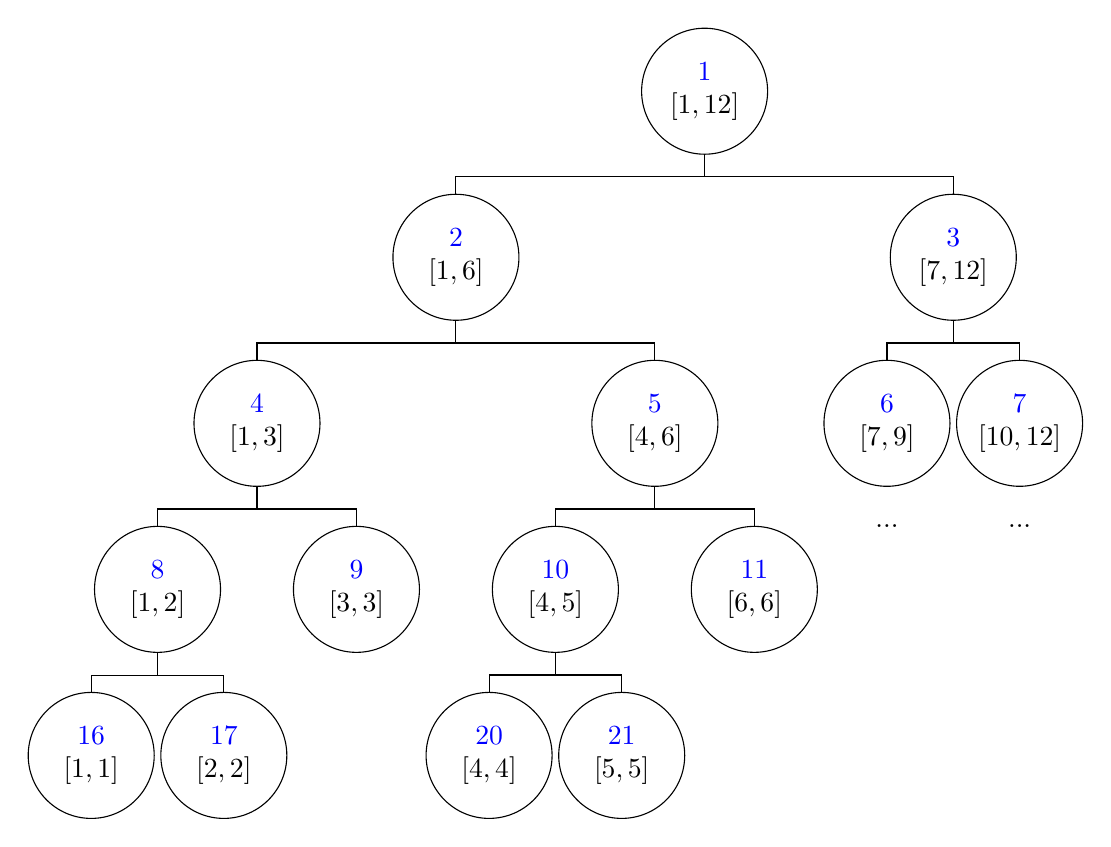
\begin{tikzpicture}[level distance=60pt]
\tikzset{edge from parent/.style=
{draw,
edge from parent path={(\tikzparentnode.south)
-- +(0,-8pt)
-| (\tikzchildnode)}}}
%\tikzset{grow'=right,level distance=32pt}
%\tikzset{execute at begin node=\strut}
%\tikzset{every tree node/.style={anchor=base west}}
\Tree
[.\node[kn](n1){{\color{blue}1}\\$[1,12]$};
  [.\node[kn]{{\color{blue}2}\\$[1,6]$};
   [.\node[kn]{{\color{blue}4}\\$[1,3]$};
    [.\node[kn]{{\color{blue}8}\\$[1,2]$};
     [.\node[kn]{{\color{blue}16}\\$[1,1]$};]
     [.\node[kn]{{\color{blue}17}\\$[2,2]$};]
    ]
    [.\node[kn]{{\color{blue}9}\\$[3,3]$};]
   ]
   [.\node[kn]{{\color{blue}5}\\$[4,6]$};
    [.\node[kn]{{\color{blue}10}\\$[4,5]$};
     [.\node[kn]{{\color{blue}20}\\$[4,4]$};]
     [.\node[kn]{{\color{blue}21}\\$[5,5]$};]
    ]
    [.\node[kn]{{\color{blue}11}\\$[6,6]$};]
   ]
  ]
  [.\node[kn]{{\color{blue}3}\\$[7,12]$};
   [.\node[kn](n6){{\color{blue}6}\\$[7,9]$};]
   [.\node[kn](n7){{\color{blue}7}\\$[10,12]$};]]
]

\node (a) at ($(n6.south) + (0, -0.5)$) {...};
\node (b) at ($(n7.south) + (0, -0.5)$) {...};
\end{tikzpicture}

	\caption{Interval tree, where the blue number in each node is the index of the node on the interval tree and the interval in each node represents the interval of the preorder sequence}
	\label{fig:3}
\end{figure}
Interval tree\footnote{\url{https://en.wikipedia.org/wiki/Interval_tree}}, is
fits for operations that aim to a continuous interval. We construct an interval
tree (Figure~\ref{fig:3}) with respect to the pre-order sequence and record each node's nearest voted parent. Each time a voter votes, we update the interval that represent the voter's child nodes in the interval tree.

We add a new global variable here.
\begin{itemize}
	\item $lazy1[2n]$: Lazy-tag in the first interval-tree\footnote{Lazy-tag is a normal operation for interval tree: when we update an interval, we can not update all the leave nodes in the interval (otherwise the time complexity is $O(n)$). Instead, we first leave the updating information to an intermediate node, that known as lazy, when next time we need to find a node included in the interval, we then sink down the lazy-tag. }
\end{itemize}

\begin{algorithm}
	\textbf{procedure} $update1(int~L,int ~R, int~l, int~r, int~k, int~v)${\color{gray}
		\\//$L,R$ are the interval for updating, and $l,r$ are node's interval,$k$ is the index of the node on interval tree, $v$ is the value for updating the interval.}
	\hrule
	\eIf {$L=l$ and $R=r$}
	{
		\If {$v>lazy1[k]$} {$lazy1[k] \leftarrow v$}
		\If {$L = R$} {$nearestparent[L] = lazy1[k]$}
		{\color{gray}
		//Recursion ends when updating interval equals to the node's interval, and then updating the value of the interval}
	}
	{
		$int~m \leftarrow (l+r)/2$\;
		\If {$lazy1[2k]<lazy[k]$} {$lazy1[2k] \leftarrow lazy1[k]$}
		\If {$lazy1[2k+1]<lazy[k]$} {$lazy1[2k+1] \leftarrow lazy1[k]${\color{gray}
			//sink down the lazy-tag}}
		\If {$L \leq m$}{$update(L,\min\{m,R\},l,m,2k,v)$}
		\If {$R>m$}{$update(\max\{m+1,L\},R,m+1,r,2k+1,v)$}
	}
\end{algorithm}
We use $update1$ to finding and update the interval tree. No extra code is needed for building the interval tree as we use $k,2k,2k+1$ to represent a node and its two children for a node in the interval tree.

The inherent property of interval tree guarantees that, there are at most two intervals in each depth that are recursively processed, so the time complexity for each updating is $O(\log n)$.

\subsection{Updating Lost Voting Power}
When a voter votes, all nodes on the path from the voter to its nearest voted parented should update their lost voting powers. See Figure \ref{fig:2}, if voter 8 votes after voter 1 votes, then path $7,3,2,1$ should be updated. However it is not a continuous interval in the pre-order sequence.
\begin{figure}
  \centering
	%\includegraphics[width=0.6\textwidth]{3.png}
  
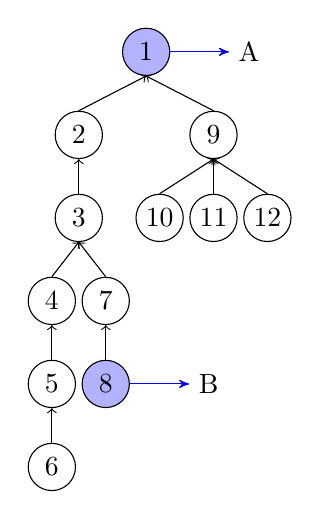
\begin{tikzpicture}
%\tikzset{grow'=right,level distance=32pt}
%\tikzset{execute at begin node=\strut}
%\tikzset{every tree node/.style={anchor=base west}}
\Tree
[.\node[fsn](n1){1};
  [.\node[sn]{2};
   [.\node[sn]{3};
    [.\node[sn]{4};
     [.\node[sn]{5};
      [.\node[sn]{6};]]]
    [.\node[sn]{7};
     [.\node[fsn](n8){8};]]] ]
  [.\node[sn]{9};
   [.\node[sn]{10};]
   [.\node[sn]{11};]
   [.\node[sn]{12};]]
]
\node (a) at ($(n1.east) + (1, 0)$) {A};
\node (b) at ($(n8.east) + (1, 0)$) {B};
\draw [->, >=stealth', color=blue] (n1) -- (a);
\draw [->, >=stealth', color=blue] (n8) -- (b);

\end{tikzpicture}

	\caption{Updating a path}
	\label{fig:2}
\end{figure}
We use the bracket sequence to handle this problem. A bracket sequence is to
record each node twice in the pre-order execution, one for enter and one for
exit, called left bracket and right bracket respectively. For Figure~\ref{fig:2}, the bracket sequence is
$$1,2,3,4,5,6,6,5,4,7,8,8,7,3,2,9,10,10,11,11,12,12,9,1$$
Let array $s[2n]$ record a value of the bracket sequence. When vote 8 votes, we let $s[1-10]+=8$, that is, the interval form node 1's left bracket to the node before node 8's left bracket.

The lost voting power of a node $u$ is $s[u.leftbracket]-s[u.rightbracket]$.

To see why, it is not hard to find that, if a node does not occur on the path we need update, it occurs twice in the interval (1-10) of the bracket sequence, say node 4,5,6. If a node is to be update, it occurs only once in the interval  (1-10) of the bracket sequence, say node 1,2,3. So from maintaining the array $s$ we can maintain each node's lost voting power. Since now the operation is an interval again, we can use another interval tree to handle it.

We add the following variables:
\begin{itemize}
%\item $s[2n]$, recording the value of the bracket sequence.
\item $lazy2[4n]$, the lazy-tag of the second interval tree.
\item $node.leftbracket,node.rightbracket$
\end{itemize}

\begin{algorithm}
	\textbf{procedure} $update2(int~L,int ~R, int~l, int~r, int~k, int~v)${\color{gray}
		\\//$L,R$ are the interval for updating, and $l,r$ are node's interval,$k$ is the index of the node on interval tree, $v$ is the value for updating the interval.}
	\hrule
	\eIf {$L=l$ and $R=r$}
	{
       $lazy2[k]+=v$
	   %\If {$L = R$} {}
	}
	{
		$int~m \leftarrow (l+r)/2$\;
		$lazy2[2k] += lazy2[k]$\;
		$lazy2[2k+1]+= lazy2[k]$\;
		$lazy2[k] \leftarrow 0$
			{\color{gray}
		//sink down the lazy-tag}\;
		\If {$L \leq m$}{$update2(L,\min\{m,R\},l,m,2k,v)$}
		\If {$R>m$}{$update2(\max\{m+1,L\},R,m+1,r,2k+1,v)$}
    }
\end{algorithm}




%\begin{algorithm}
%	\textbf{Procedure} $Build(int~k,int~l,int ~r)$;

%\end{algorithm}





\end{document}
